\documentclass[1p]{elsarticle_modified}
%\bibliographystyle{elsarticle-num}

%\usepackage[colorlinks]{hyperref}
%\usepackage{abbrmath_seonhwa} %\Abb, \Ascr, \Acal ,\Abf, \Afrak
\usepackage{amsfonts}
\usepackage{amssymb}
\usepackage{amsmath}
\usepackage{amsthm}
\usepackage{scalefnt}
\usepackage{amsbsy}
\usepackage{kotex}
\usepackage{caption}
\usepackage{subfig}
\usepackage{color}
\usepackage{graphicx}
\usepackage{xcolor} %% white, black, red, green, blue, cyan, magenta, yellow
\usepackage{float}
\usepackage{setspace}
\usepackage{hyperref}

\usepackage{tikz}
\usetikzlibrary{arrows}

\usepackage{multirow}
\usepackage{array} % fixed length table
\usepackage{hhline}

%%%%%%%%%%%%%%%%%%%%%
\makeatletter
\renewcommand*\env@matrix[1][\arraystretch]{%
	\edef\arraystretch{#1}%
	\hskip -\arraycolsep
	\let\@ifnextchar\new@ifnextchar
	\array{*\c@MaxMatrixCols c}}
\makeatother %https://tex.stackexchange.com/questions/14071/how-can-i-increase-the-line-spacing-in-a-matrix
%%%%%%%%%%%%%%%

\usepackage[normalem]{ulem}

\newcommand{\msout}[1]{\ifmmode\text{\sout{\ensuremath{#1}}}\else\sout{#1}\fi}
%SOURCE: \msout is \stkout macro in https://tex.stackexchange.com/questions/20609/strikeout-in-math-mode

\newcommand{\cancel}[1]{
	\ifmmode
	{\color{red}\msout{#1}}
	\else
	{\color{red}\sout{#1}}
	\fi
}

\newcommand{\add}[1]{
	{\color{blue}\uwave{#1}}
}

\newcommand{\replace}[2]{
	\ifmmode
	{\color{red}\msout{#1}}{\color{blue}\uwave{#2}}
	\else
	{\color{red}\sout{#1}}{\color{blue}\uwave{#2}}
	\fi
}

\newcommand{\Sol}{\mathcal{S}} %segment
\newcommand{\D}{D} %diagram
\newcommand{\A}{\mathcal{A}} %arc


%%%%%%%%%%%%%%%%%%%%%%%%%%%%%5 test

\def\sl{\operatorname{\textup{SL}}(2,\Cbb)}
\def\psl{\operatorname{\textup{PSL}}(2,\Cbb)}
\def\quan{\mkern 1mu \triangleright \mkern 1mu}

\theoremstyle{definition}
\newtheorem{thm}{Theorem}[section]
\newtheorem{prop}[thm]{Proposition}
\newtheorem{lem}[thm]{Lemma}
\newtheorem{ques}[thm]{Question}
\newtheorem{cor}[thm]{Corollary}
\newtheorem{defn}[thm]{Definition}
\newtheorem{exam}[thm]{Example}
\newtheorem{rmk}[thm]{Remark}
\newtheorem{alg}[thm]{Algorithm}

\newcommand{\I}{\sqrt{-1}}
\begin{document}

%\begin{frontmatter}
%
%\title{Boundary parabolic representations of knots up to 8 crossings}
%
%%% Group authors per affiliation:
%\author{Yunhi Cho} 
%\address{Department of Mathematics, University of Seoul, Seoul, Korea}
%\ead{yhcho@uos.ac.kr}
%
%
%\author{Seonhwa Kim} %\fnref{s_kim}}
%\address{Center for Geometry and Physics, Institute for Basic Science, Pohang, 37673, Korea}
%\ead{ryeona17@ibs.re.kr}
%
%\author{Hyuk Kim}
%\address{Department of Mathematical Sciences, Seoul National University, Seoul 08826, Korea}
%\ead{hyukkim@snu.ac.kr}
%
%\author{Seokbeom Yoon}
%\address{Department of Mathematical Sciences, Seoul National University, Seoul, 08826,  Korea}
%\ead{sbyoon15@snu.ac.kr}
%
%\begin{abstract}
%We find all boundary parabolic representation of knots up to 8 crossings.
%
%\end{abstract}
%\begin{keyword}
%    \MSC[2010] 57M25 
%\end{keyword}
%
%\end{frontmatter}

%\linenumbers
%\tableofcontents
%
\newcommand\colored[1]{\textcolor{white}{\rule[-0.35ex]{0.8em}{1.4ex}}\kern-0.8em\color{red} #1}%
%\newcommand\colored[1]{\textcolor{white}{ #1}\kern-2.17ex	\textcolor{white}{ #1}\kern-1.81ex	\textcolor{white}{ #1}\kern-2.15ex\color{red}#1	}

{\Large $\underline{12a_{0273}~(K12a_{0273})}$}

\setlength{\tabcolsep}{10pt}
\renewcommand{\arraystretch}{1.6}
\vspace{1cm}\begin{tabular}{m{100pt}>{\centering\arraybackslash}m{274pt}}
\multirow{5}{120pt}{
	\centering
	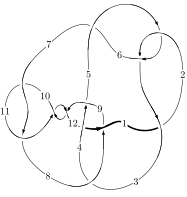
\includegraphics[width=112pt]{../../../GIT/diagram.site/Diagrams/png/1074_12a_0273.png}\\
\ \ \ A knot diagram\footnotemark}&
\allowdisplaybreaks
\textbf{Linearized knot diagam} \\
\cline{2-2}
 &
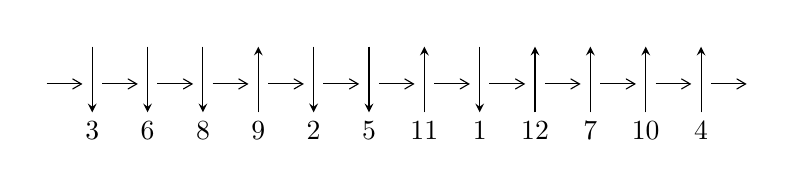
\begin{tikzpicture}[x=20pt, y=17pt]
	% nodes
	\node (C0) at (0, 0) {};
	\node (C1) at (1, 0) {};
	\node (C1U) at (1, +1) {};
	\node (C1D) at (1, -1) {3};

	\node (C2) at (2, 0) {};
	\node (C2U) at (2, +1) {};
	\node (C2D) at (2, -1) {6};

	\node (C3) at (3, 0) {};
	\node (C3U) at (3, +1) {};
	\node (C3D) at (3, -1) {8};

	\node (C4) at (4, 0) {};
	\node (C4U) at (4, +1) {};
	\node (C4D) at (4, -1) {9};

	\node (C5) at (5, 0) {};
	\node (C5U) at (5, +1) {};
	\node (C5D) at (5, -1) {2};

	\node (C6) at (6, 0) {};
	\node (C6U) at (6, +1) {};
	\node (C6D) at (6, -1) {5};

	\node (C7) at (7, 0) {};
	\node (C7U) at (7, +1) {};
	\node (C7D) at (7, -1) {11};

	\node (C8) at (8, 0) {};
	\node (C8U) at (8, +1) {};
	\node (C8D) at (8, -1) {1};

	\node (C9) at (9, 0) {};
	\node (C9U) at (9, +1) {};
	\node (C9D) at (9, -1) {12};

	\node (C10) at (10, 0) {};
	\node (C10U) at (10, +1) {};
	\node (C10D) at (10, -1) {7};

	\node (C11) at (11, 0) {};
	\node (C11U) at (11, +1) {};
	\node (C11D) at (11, -1) {10};

	\node (C12) at (12, 0) {};
	\node (C12U) at (12, +1) {};
	\node (C12D) at (12, -1) {4};
	\node (C13) at (13, 0) {};

	% arrows
	\draw[->,>={angle 60}]
	(C0) edge (C1) (C1) edge (C2) (C2) edge (C3) (C3) edge (C4) (C4) edge (C5) (C5) edge (C6) (C6) edge (C7) (C7) edge (C8) (C8) edge (C9) (C9) edge (C10) (C10) edge (C11) (C11) edge (C12) (C12) edge (C13) ;	\draw[->,>=stealth]
	(C1U) edge (C1D) (C2U) edge (C2D) (C3U) edge (C3D) (C4D) edge (C4U) (C5U) edge (C5D) (C6U) edge (C6D) (C7D) edge (C7U) (C8U) edge (C8D) (C9D) edge (C9U) (C10D) edge (C10U) (C11D) edge (C11U) (C12D) edge (C12U) ;
	\end{tikzpicture} \\
\hhline{~~} \\& 
\textbf{Solving Sequence} \\ \cline{2-2} 
 &
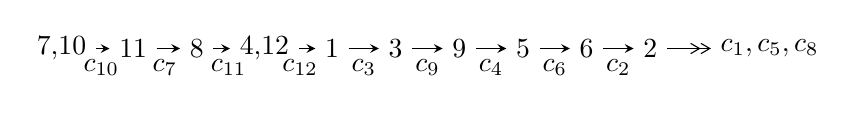
\begin{tikzpicture}[x=23pt, y=7pt]
	% node
	\node (A0) at (-1/8, 0) {7,10};
	\node (A1) at (1, 0) {11};
	\node (A2) at (2, 0) {8};
	\node (A3) at (49/16, 0) {4,12};
	\node (A4) at (33/8, 0) {1};
	\node (A5) at (41/8, 0) {3};
	\node (A6) at (49/8, 0) {9};
	\node (A7) at (57/8, 0) {5};
	\node (A8) at (65/8, 0) {6};
	\node (A9) at (73/8, 0) {2};
	\node (C1) at (1/2, -1) {$c_{10}$};
	\node (C2) at (3/2, -1) {$c_{7}$};
	\node (C3) at (5/2, -1) {$c_{11}$};
	\node (C4) at (29/8, -1) {$c_{12}$};
	\node (C5) at (37/8, -1) {$c_{3}$};
	\node (C6) at (45/8, -1) {$c_{9}$};
	\node (C7) at (53/8, -1) {$c_{4}$};
	\node (C8) at (61/8, -1) {$c_{6}$};
	\node (C9) at (69/8, -1) {$c_{2}$};
	\node (A10) at (11, 0) {$c_{1},c_{5},c_{8}$};

	% edge
	\draw[->,>=stealth]	
	(A0) edge (A1) (A1) edge (A2) (A2) edge (A3) (A3) edge (A4) (A4) edge (A5) (A5) edge (A6) (A6) edge (A7) (A7) edge (A8) (A8) edge (A9) ;
	\draw[->>,>={angle 60}]	
	(A9) edge (A10);
\end{tikzpicture} \\ 

\end{tabular} \\

\footnotetext{
The image of knot diagram is generated by the software ``\textbf{Draw programme}" developed by Andrew Bartholomew(\url{http://www.layer8.co.uk/maths/draw/index.htm\#Running-draw}), where we modified some parts for our purpose(\url{https://github.com/CATsTAILs/LinksPainter}).
}\phantom \\ \newline 
\centering \textbf{Ideals for irreducible components\footnotemark of $X_{\text{par}}$} 
 
\begin{align*}
I^u_{1}&=\langle 
4.11782\times10^{111} u^{107}-1.72896\times10^{112} u^{106}+\cdots+2.70657\times10^{109} b+5.15017\times10^{111},\\
\phantom{I^u_{1}}&\phantom{= \langle  }-9.18604\times10^{110} u^{107}+3.85195\times10^{111} u^{106}+\cdots+1.35329\times10^{109} a-1.19005\times10^{111},\\
\phantom{I^u_{1}}&\phantom{= \langle  }u^{108}-5 u^{107}+\cdots-4 u-1\rangle \\
I^u_{2}&=\langle 
b^3- b^2+2 b-1,\;a,\;u-1\rangle \\
I^u_{3}&=\langle 
b,\;a- u-1,\;u^3+u^2-1\rangle \\
\\
\end{align*}
\raggedright * 3 irreducible components of $\dim_{\mathbb{C}}=0$, with total 114 representations.\\
\footnotetext{All coefficients of polynomials are rational numbers. But the coefficients are sometimes approximated in decimal forms when there is not enough margin.}
\newpage
\renewcommand{\arraystretch}{1}
\centering \section*{I. $I^u_{1}= \langle 4.12\times10^{111} u^{107}-1.73\times10^{112} u^{106}+\cdots+2.71\times10^{109} b+5.15\times10^{111},\;-9.19\times10^{110} u^{107}+3.85\times10^{111} u^{106}+\cdots+1.35\times10^{109} a-1.19\times10^{111},\;u^{108}-5 u^{107}+\cdots-4 u-1 \rangle$}
\flushleft \textbf{(i) Arc colorings}\\
\begin{tabular}{m{7pt} m{180pt} m{7pt} m{180pt} }
\flushright $a_{7}=$&$\begin{pmatrix}0\\u\end{pmatrix}$ \\
\flushright $a_{10}=$&$\begin{pmatrix}1\\0\end{pmatrix}$ \\
\flushright $a_{11}=$&$\begin{pmatrix}1\\- u^2\end{pmatrix}$ \\
\flushright $a_{8}=$&$\begin{pmatrix}u\\- u^3+u\end{pmatrix}$ \\
\flushright $a_{4}=$&$\begin{pmatrix}67.8795 u^{107}-284.637 u^{106}+\cdots+399.400 u+87.9382\\-152.142 u^{107}+638.802 u^{106}+\cdots-1002.39 u-190.284\end{pmatrix}$ \\
\flushright $a_{12}=$&$\begin{pmatrix}- u^2+1\\- u^2\end{pmatrix}$ \\
\flushright $a_{1}=$&$\begin{pmatrix}6.01771 u^{107}-24.3208 u^{106}+\cdots+36.1965 u+2.67705\\-5.22248 u^{107}+26.6576 u^{106}+\cdots-58.8780 u-11.2402\end{pmatrix}$ \\
\flushright $a_{3}=$&$\begin{pmatrix}-48.5904 u^{107}+202.556 u^{106}+\cdots-350.712 u-55.3704\\-190.876 u^{107}+800.455 u^{106}+\cdots-1255.40 u-238.436\end{pmatrix}$ \\
\flushright $a_{9}=$&$\begin{pmatrix}u^4- u^2+1\\u^4\end{pmatrix}$ \\
\flushright $a_{5}=$&$\begin{pmatrix}-48.3647 u^{107}+201.869 u^{106}+\cdots-350.353 u-54.7783\\-216.521 u^{107}+905.574 u^{106}+\cdots-1403.65 u-267.141\end{pmatrix}$ \\
\flushright $a_{6}=$&$\begin{pmatrix}16.3787 u^{107}-67.4197 u^{106}+\cdots+101.379 u+11.9449\\46.8149 u^{107}-192.264 u^{106}+\cdots+275.135 u+52.5332\end{pmatrix}$ \\
\flushright $a_{2}=$&$\begin{pmatrix}-12.7836 u^{107}+52.3966 u^{106}+\cdots-69.4987 u-11.0363\\-42.8242 u^{107}+178.501 u^{106}+\cdots-268.820 u-51.4147\end{pmatrix}$\\&\end{tabular}
\flushleft \textbf{(ii) Obstruction class $= -1$}\\~\\
\flushleft \textbf{(iii) Cusp Shapes $= -359.027 u^{107}+1549.26 u^{106}+\cdots-2737.10 u-515.927$}\\~\\
\newpage\renewcommand{\arraystretch}{1}
\flushleft \textbf{(iv) u-Polynomials at the component}\newline \\
\begin{tabular}{m{50pt}|m{274pt}}
Crossings & \hspace{64pt}u-Polynomials at each crossing \\
\hline $$\begin{aligned}c_{1},c_{6}\end{aligned}$$&$\begin{aligned}
&u^{108}+35 u^{107}+\cdots+146 u+1
\end{aligned}$\\
\hline $$\begin{aligned}c_{2},c_{5}\end{aligned}$$&$\begin{aligned}
&u^{108}+5 u^{107}+\cdots+4 u-1
\end{aligned}$\\
\hline $$\begin{aligned}c_{3}\end{aligned}$$&$\begin{aligned}
&u^{108}+u^{107}+\cdots-163 u-383
\end{aligned}$\\
\hline $$\begin{aligned}c_{4}\end{aligned}$$&$\begin{aligned}
&u^{108}- u^{107}+\cdots+163 u-383
\end{aligned}$\\
\hline $$\begin{aligned}c_{7},c_{10}\end{aligned}$$&$\begin{aligned}
&u^{108}-5 u^{107}+\cdots-4 u-1
\end{aligned}$\\
\hline $$\begin{aligned}c_{8}\end{aligned}$$&$\begin{aligned}
&u^{108}-10 u^{107}+\cdots-12 u+8
\end{aligned}$\\
\hline $$\begin{aligned}c_{9},c_{11}\end{aligned}$$&$\begin{aligned}
&u^{108}-35 u^{107}+\cdots-146 u+1
\end{aligned}$\\
\hline $$\begin{aligned}c_{12}\end{aligned}$$&$\begin{aligned}
&u^{108}+10 u^{107}+\cdots+12 u+8
\end{aligned}$\\
\hline
\end{tabular}\\~\\
\newpage\renewcommand{\arraystretch}{1}
\flushleft \textbf{(v) Riley Polynomials at the component}\newline \\
\begin{tabular}{m{50pt}|m{274pt}}
Crossings & \hspace{64pt}Riley Polynomials at each crossing \\
\hline $$\begin{aligned}c_{1},c_{6},c_{9}\\c_{11}\end{aligned}$$&$\begin{aligned}
&y^{108}+81 y^{107}+\cdots-19954 y+1
\end{aligned}$\\
\hline $$\begin{aligned}c_{2},c_{5},c_{7}\\c_{10}\end{aligned}$$&$\begin{aligned}
&y^{108}-35 y^{107}+\cdots-146 y+1
\end{aligned}$\\
\hline $$\begin{aligned}c_{3},c_{4}\end{aligned}$$&$\begin{aligned}
&y^{108}+123 y^{107}+\cdots-3629833 y+146689
\end{aligned}$\\
\hline $$\begin{aligned}c_{8},c_{12}\end{aligned}$$&$\begin{aligned}
&y^{108}+18 y^{107}+\cdots+1904 y+64
\end{aligned}$\\
\hline
\end{tabular}\\~\\
\newpage\flushleft \textbf{(vi) Complex Volumes and Cusp Shapes}
$$\begin{array}{c|c|c}  
\text{Solutions to }I^u_{1}& \I (\text{vol} + \sqrt{-1}CS) & \text{Cusp shape}\\
 \hline 
\begin{aligned}
u &= -0.979728 + 0.166940 I \\
a &= -1.038070 + 0.480900 I \\
b &= \phantom{-}0.136075 + 0.665202 I\end{aligned}
 & \phantom{-}3.19306 - 3.71797 I & \phantom{-0.000000 } 0 \\ \hline\begin{aligned}
u &= -0.979728 - 0.166940 I \\
a &= -1.038070 - 0.480900 I \\
b &= \phantom{-}0.136075 - 0.665202 I\end{aligned}
 & \phantom{-}3.19306 + 3.71797 I & \phantom{-0.000000 } 0 \\ \hline\begin{aligned}
u &= -0.605005 + 0.787681 I \\
a &= \phantom{-}0.845635 - 0.095086 I \\
b &= \phantom{-}0.962946 + 0.612440 I\end{aligned}
 & -2.14715 - 1.03507 I & \phantom{-0.000000 } 0 \\ \hline\begin{aligned}
u &= -0.605005 - 0.787681 I \\
a &= \phantom{-}0.845635 + 0.095086 I \\
b &= \phantom{-}0.962946 - 0.612440 I\end{aligned}
 & -2.14715 + 1.03507 I & \phantom{-0.000000 } 0 \\ \hline\begin{aligned}
u &= \phantom{-}0.715108 + 0.670386 I \\
a &= \phantom{-}0.771317 + 0.384628 I \\
b &= \phantom{-}0.157147 - 1.104620 I\end{aligned}
 & \phantom{-}2.14715 + 1.03507 I & \phantom{-0.000000 } 0 \\ \hline\begin{aligned}
u &= \phantom{-}0.715108 - 0.670386 I \\
a &= \phantom{-}0.771317 - 0.384628 I \\
b &= \phantom{-}0.157147 + 1.104620 I\end{aligned}
 & \phantom{-}2.14715 - 1.03507 I & \phantom{-0.000000 } 0 \\ \hline\begin{aligned}
u &= -0.973353 + 0.047519 I \\
a &= -1.02470 - 1.12942 I \\
b &= -0.075717 - 1.064180 I\end{aligned}
 & \phantom{-}7.14796 + 0.81738 I & \phantom{-0.000000 } 0 \\ \hline\begin{aligned}
u &= -0.973353 - 0.047519 I \\
a &= -1.02470 + 1.12942 I \\
b &= -0.075717 + 1.064180 I\end{aligned}
 & \phantom{-}7.14796 - 0.81738 I & \phantom{-0.000000 } 0 \\ \hline\begin{aligned}
u &= -0.956601 + 0.099212 I \\
a &= \phantom{-}0.99426 + 1.23398 I \\
b &= \phantom{-}0.124520 + 1.135330 I\end{aligned}
 & \phantom{-}6.35502 - 5.36585 I & \phantom{-0.000000 } 0 \\ \hline\begin{aligned}
u &= -0.956601 - 0.099212 I \\
a &= \phantom{-}0.99426 - 1.23398 I \\
b &= \phantom{-}0.124520 - 1.135330 I\end{aligned}
 & \phantom{-}6.35502 + 5.36585 I & \phantom{-0.000000 } 0\\
 \hline 
 \end{array}$$\newpage$$\begin{array}{c|c|c}  
\text{Solutions to }I^u_{1}& \I (\text{vol} + \sqrt{-1}CS) & \text{Cusp shape}\\
 \hline 
\begin{aligned}
u &= \phantom{-}0.745810 + 0.744346 I \\
a &= -1.027490 - 0.410866 I \\
b &= -0.451934 + 1.247910 I\end{aligned}
 & \phantom{-}0.82383 - 4.62628 I & \phantom{-0.000000 } 0 \\ \hline\begin{aligned}
u &= \phantom{-}0.745810 - 0.744346 I \\
a &= -1.027490 + 0.410866 I \\
b &= -0.451934 - 1.247910 I\end{aligned}
 & \phantom{-}0.82383 + 4.62628 I & \phantom{-0.000000 } 0 \\ \hline\begin{aligned}
u &= \phantom{-}0.850637 + 0.406962 I \\
a &= \phantom{-}0.080872 + 0.341351 I \\
b &= -0.238152 - 0.726384 I\end{aligned}
 & \phantom{-}1.82900 + 1.35958 I & \phantom{-0.000000 } 0 \\ \hline\begin{aligned}
u &= \phantom{-}0.850637 - 0.406962 I \\
a &= \phantom{-}0.080872 - 0.341351 I \\
b &= -0.238152 + 0.726384 I\end{aligned}
 & \phantom{-}1.82900 - 1.35958 I & \phantom{-0.000000 } 0 \\ \hline\begin{aligned}
u &= -1.019000 + 0.284607 I \\
a &= \phantom{-}0.769824 - 0.155699 I \\
b &= -0.374588 - 0.510091 I\end{aligned}
 & \phantom{-0.000000 } -7.09355 I & \phantom{-0.000000 } 0 \\ \hline\begin{aligned}
u &= -1.019000 - 0.284607 I \\
a &= \phantom{-}0.769824 + 0.155699 I \\
b &= -0.374588 + 0.510091 I\end{aligned}
 & \phantom{-0.000000 -}7.09355 I & \phantom{-0.000000 } 0 \\ \hline\begin{aligned}
u &= \phantom{-}0.862762 + 0.622752 I \\
a &= -1.58251 - 1.51375 I \\
b &= -2.86284 + 0.83647 I\end{aligned}
 & \phantom{-}3.75903 - 0.77126 I & \phantom{-0.000000 } 0 \\ \hline\begin{aligned}
u &= \phantom{-}0.862762 - 0.622752 I \\
a &= -1.58251 + 1.51375 I \\
b &= -2.86284 - 0.83647 I\end{aligned}
 & \phantom{-}3.75903 + 0.77126 I & \phantom{-0.000000 } 0 \\ \hline\begin{aligned}
u &= -0.616674 + 0.874327 I \\
a &= -0.865658 + 0.308655 I \\
b &= -1.042850 - 0.462236 I\end{aligned}
 & -2.85537 + 4.21466 I & \phantom{-0.000000 } 0 \\ \hline\begin{aligned}
u &= -0.616674 - 0.874327 I \\
a &= -0.865658 - 0.308655 I \\
b &= -1.042850 + 0.462236 I\end{aligned}
 & -2.85537 - 4.21466 I & \phantom{-0.000000 } 0\\
 \hline 
 \end{array}$$\newpage$$\begin{array}{c|c|c}  
\text{Solutions to }I^u_{1}& \I (\text{vol} + \sqrt{-1}CS) & \text{Cusp shape}\\
 \hline 
\begin{aligned}
u &= -0.814404 + 0.714383 I \\
a &= \phantom{-}1.00553 + 2.14684 I \\
b &= -0.52002 + 1.34231 I\end{aligned}
 & \phantom{-0.000000 } -4.57359 I & \phantom{-0.000000 } 0 \\ \hline\begin{aligned}
u &= -0.814404 - 0.714383 I \\
a &= \phantom{-}1.00553 - 2.14684 I \\
b &= -0.52002 - 1.34231 I\end{aligned}
 & \phantom{-0.000000 -}4.57359 I & \phantom{-0.000000 } 0 \\ \hline\begin{aligned}
u &= \phantom{-}0.744550 + 0.799387 I \\
a &= -1.43674 - 1.59030 I \\
b &= -2.50978 - 0.05086 I\end{aligned}
 & -3.11037 - 2.87230 I & \phantom{-0.000000 } 0 \\ \hline\begin{aligned}
u &= \phantom{-}0.744550 - 0.799387 I \\
a &= -1.43674 + 1.59030 I \\
b &= -2.50978 + 0.05086 I\end{aligned}
 & -3.11037 + 2.87230 I & \phantom{-0.000000 } 0 \\ \hline\begin{aligned}
u &= \phantom{-}0.907254 + 0.638959 I \\
a &= \phantom{-}1.66458 + 1.44541 I \\
b &= \phantom{-}2.94097 - 0.92211 I\end{aligned}
 & \phantom{-}3.93257 + 5.67737 I & \phantom{-0.000000 } 0 \\ \hline\begin{aligned}
u &= \phantom{-}0.907254 - 0.638959 I \\
a &= \phantom{-}1.66458 - 1.44541 I \\
b &= \phantom{-}2.94097 + 0.92211 I\end{aligned}
 & \phantom{-}3.93257 - 5.67737 I & \phantom{-0.000000 } 0 \\ \hline\begin{aligned}
u &= -0.821570 + 0.746772 I \\
a &= -1.20102 - 2.36279 I \\
b &= \phantom{-}0.40213 - 1.66223 I\end{aligned}
 & -0.298325 + 0.873313 I & \phantom{-0.000000 } 0 \\ \hline\begin{aligned}
u &= -0.821570 - 0.746772 I \\
a &= -1.20102 + 2.36279 I \\
b &= \phantom{-}0.40213 + 1.66223 I\end{aligned}
 & -0.298325 - 0.873313 I & \phantom{-0.000000 } 0 \\ \hline\begin{aligned}
u &= \phantom{-}0.693031 + 0.877224 I \\
a &= -1.53841 - 1.50089 I \\
b &= -2.30877 - 0.13072 I\end{aligned}
 & \phantom{-0.000000 } -6.29181 I & \phantom{-0.000000 } 0 \\ \hline\begin{aligned}
u &= \phantom{-}0.693031 - 0.877224 I \\
a &= -1.53841 + 1.50089 I \\
b &= -2.30877 + 0.13072 I\end{aligned}
 & \phantom{-0.000000 -}6.29181 I & \phantom{-0.000000 } 0\\
 \hline 
 \end{array}$$\newpage$$\begin{array}{c|c|c}  
\text{Solutions to }I^u_{1}& \I (\text{vol} + \sqrt{-1}CS) & \text{Cusp shape}\\
 \hline 
\begin{aligned}
u &= \phantom{-}0.870551 + 0.703926 I \\
a &= -0.881042 + 0.605315 I \\
b &= \phantom{-}0.58910 + 2.04797 I\end{aligned}
 & -3.89287 + 2.70030 I & \phantom{-0.000000 } 0 \\ \hline\begin{aligned}
u &= \phantom{-}0.870551 - 0.703926 I \\
a &= -0.881042 - 0.605315 I \\
b &= \phantom{-}0.58910 - 2.04797 I\end{aligned}
 & -3.89287 - 2.70030 I & \phantom{-0.000000 } 0 \\ \hline\begin{aligned}
u &= -0.816700 + 0.769783 I \\
a &= \phantom{-}1.72760 - 0.26942 I \\
b &= \phantom{-}1.63286 + 0.89494 I\end{aligned}
 & -3.53829 - 1.78224 I & \phantom{-0.000000 } 0 \\ \hline\begin{aligned}
u &= -0.816700 - 0.769783 I \\
a &= \phantom{-}1.72760 + 0.26942 I \\
b &= \phantom{-}1.63286 - 0.89494 I\end{aligned}
 & -3.53829 + 1.78224 I & \phantom{-0.000000 } 0 \\ \hline\begin{aligned}
u &= \phantom{-}0.803722 + 0.787733 I \\
a &= \phantom{-}1.32736 + 1.65587 I \\
b &= \phantom{-}2.73483 + 0.18727 I\end{aligned}
 & -6.28442 + 1.49926 I & \phantom{-0.000000 } 0 \\ \hline\begin{aligned}
u &= \phantom{-}0.803722 - 0.787733 I \\
a &= \phantom{-}1.32736 - 1.65587 I \\
b &= \phantom{-}2.73483 - 0.18727 I\end{aligned}
 & -6.28442 - 1.49926 I & \phantom{-0.000000 } 0 \\ \hline\begin{aligned}
u &= \phantom{-}1.112550 + 0.201315 I \\
a &= \phantom{-}0.154894 - 0.326872 I \\
b &= \phantom{-}0.202520 + 0.144144 I\end{aligned}
 & \phantom{-}0.629927 - 0.566671 I & \phantom{-0.000000 } 0 \\ \hline\begin{aligned}
u &= \phantom{-}1.112550 - 0.201315 I \\
a &= \phantom{-}0.154894 + 0.326872 I \\
b &= \phantom{-}0.202520 - 0.144144 I\end{aligned}
 & \phantom{-}0.629927 + 0.566671 I & \phantom{-0.000000 } 0 \\ \hline\begin{aligned}
u &= \phantom{-}0.866946\phantom{ +0.000000I} \\
a &= \phantom{-}0.530489\phantom{ +0.000000I} \\
b &= -0.445872\phantom{ +0.000000I}\end{aligned}
 & \phantom{-}1.43135\phantom{ +0.000000I} & \phantom{-0.000000 } 0 \\ \hline\begin{aligned}
u &= \phantom{-}0.700693 + 0.895805 I \\
a &= \phantom{-}1.54343 + 1.47096 I \\
b &= \phantom{-}2.30224 + 0.16065 I\end{aligned}
 & -1.06026 - 12.34350 I & \phantom{-0.000000 } 0\\
 \hline 
 \end{array}$$\newpage$$\begin{array}{c|c|c}  
\text{Solutions to }I^u_{1}& \I (\text{vol} + \sqrt{-1}CS) & \text{Cusp shape}\\
 \hline 
\begin{aligned}
u &= \phantom{-}0.700693 - 0.895805 I \\
a &= \phantom{-}1.54343 - 1.47096 I \\
b &= \phantom{-}2.30224 - 0.16065 I\end{aligned}
 & -1.06026 + 12.34350 I & \phantom{-0.000000 } 0 \\ \hline\begin{aligned}
u &= \phantom{-}0.752822 + 0.857130 I \\
a &= \phantom{-}1.43527 + 1.49045 I \\
b &= \phantom{-}2.41571 + 0.18143 I\end{aligned}
 & -7.40743 - 6.11835 I & \phantom{-0.000000 } 0 \\ \hline\begin{aligned}
u &= \phantom{-}0.752822 - 0.857130 I \\
a &= \phantom{-}1.43527 - 1.49045 I \\
b &= \phantom{-}2.41571 - 0.18143 I\end{aligned}
 & -7.40743 + 6.11835 I & \phantom{-0.000000 } 0 \\ \hline\begin{aligned}
u &= -1.126570 + 0.214725 I \\
a &= -0.564137 + 0.491665 I \\
b &= \phantom{-}0.450345 + 0.778573 I\end{aligned}
 & \phantom{-}7.40743 - 6.11835 I & \phantom{-0.000000 } 0 \\ \hline\begin{aligned}
u &= -1.126570 - 0.214725 I \\
a &= -0.564137 - 0.491665 I \\
b &= \phantom{-}0.450345 - 0.778573 I\end{aligned}
 & \phantom{-}7.40743 + 6.11835 I & \phantom{-0.000000 } 0 \\ \hline\begin{aligned}
u &= \phantom{-}0.107937 + 0.844817 I \\
a &= -0.365482 - 0.693695 I \\
b &= \phantom{-}0.131212 + 0.293224 I\end{aligned}
 & \phantom{-}2.38418 + 8.65987 I & \phantom{-0.000000 } 0 \\ \hline\begin{aligned}
u &= \phantom{-}0.107937 - 0.844817 I \\
a &= -0.365482 + 0.693695 I \\
b &= \phantom{-}0.131212 - 0.293224 I\end{aligned}
 & \phantom{-}2.38418 - 8.65987 I & \phantom{-0.000000 } 0 \\ \hline\begin{aligned}
u &= -0.912663 + 0.707599 I \\
a &= \phantom{-}2.08182 + 1.46268 I \\
b &= \phantom{-}0.95698 + 2.07662 I\end{aligned}
 & \phantom{-}0.298325 - 0.873313 I & \phantom{-0.000000 } 0 \\ \hline\begin{aligned}
u &= -0.912663 - 0.707599 I \\
a &= \phantom{-}2.08182 - 1.46268 I \\
b &= \phantom{-}0.95698 - 2.07662 I\end{aligned}
 & \phantom{-}0.298325 + 0.873313 I & \phantom{-0.000000 } 0 \\ \hline\begin{aligned}
u &= -0.878636 + 0.753546 I \\
a &= -2.34831 - 3.13274 I \\
b &= \phantom{-}0.00650 - 3.16279 I\end{aligned}
 & -4.37927 - 2.85474 I & \phantom{-0.000000 } 0\\
 \hline 
 \end{array}$$\newpage$$\begin{array}{c|c|c}  
\text{Solutions to }I^u_{1}& \I (\text{vol} + \sqrt{-1}CS) & \text{Cusp shape}\\
 \hline 
\begin{aligned}
u &= -0.878636 - 0.753546 I \\
a &= -2.34831 + 3.13274 I \\
b &= \phantom{-}0.00650 + 3.16279 I\end{aligned}
 & -4.37927 + 2.85474 I & \phantom{-0.000000 } 0 \\ \hline\begin{aligned}
u &= -0.752213 + 0.881864 I \\
a &= -1.149800 + 0.436361 I \\
b &= -1.329100 - 0.473314 I\end{aligned}
 & -7.14796 - 0.81738 I & \phantom{-0.000000 } 0 \\ \hline\begin{aligned}
u &= -0.752213 - 0.881864 I \\
a &= -1.149800 - 0.436361 I \\
b &= -1.329100 + 0.473314 I\end{aligned}
 & -7.14796 + 0.81738 I & \phantom{-0.000000 } 0 \\ \hline\begin{aligned}
u &= -1.140280 + 0.239475 I \\
a &= \phantom{-}0.499762 - 0.446388 I \\
b &= -0.505072 - 0.759246 I\end{aligned}
 & \phantom{-}6.64063 - 12.17460 I & \phantom{-0.000000 } 0 \\ \hline\begin{aligned}
u &= -1.140280 - 0.239475 I \\
a &= \phantom{-}0.499762 + 0.446388 I \\
b &= -0.505072 + 0.759246 I\end{aligned}
 & \phantom{-}6.64063 + 12.17460 I & \phantom{-0.000000 } 0 \\ \hline\begin{aligned}
u &= \phantom{-}0.829074 + 0.011014 I \\
a &= -0.07425 - 1.42512 I \\
b &= -0.16570 + 4.05652 I\end{aligned}
 & \phantom{-}4.37927 + 2.85474 I & \phantom{-0.000000 } 0 \\ \hline\begin{aligned}
u &= \phantom{-}0.829074 - 0.011014 I \\
a &= -0.07425 + 1.42512 I \\
b &= -0.16570 - 4.05652 I\end{aligned}
 & \phantom{-}4.37927 - 2.85474 I & \phantom{-0.000000 } 0 \\ \hline\begin{aligned}
u &= -0.918379 + 0.727605 I \\
a &= -2.14206 - 1.70389 I \\
b &= -0.85806 - 2.22807 I\end{aligned}
 & \phantom{-0.000000 } -6.47878 I & \phantom{-0.000000 } 0 \\ \hline\begin{aligned}
u &= -0.918379 - 0.727605 I \\
a &= -2.14206 + 1.70389 I \\
b &= -0.85806 + 2.22807 I\end{aligned}
 & \phantom{-0.000000 -}6.47878 I & \phantom{-0.000000 } 0 \\ \hline\begin{aligned}
u &= -0.819143 + 0.114490 I \\
a &= \phantom{-}1.78431 - 0.53842 I \\
b &= \phantom{-}0.292058 - 0.533870 I\end{aligned}
 & -0.629927 - 0.566671 I & \phantom{-0.000000 } 0\\
 \hline 
 \end{array}$$\newpage$$\begin{array}{c|c|c}  
\text{Solutions to }I^u_{1}& \I (\text{vol} + \sqrt{-1}CS) & \text{Cusp shape}\\
 \hline 
\begin{aligned}
u &= -0.819143 - 0.114490 I \\
a &= \phantom{-}1.78431 + 0.53842 I \\
b &= \phantom{-}0.292058 + 0.533870 I\end{aligned}
 & -0.629927 + 0.566671 I & \phantom{-0.000000 } 0 \\ \hline\begin{aligned}
u &= \phantom{-}0.958471 + 0.677586 I \\
a &= \phantom{-}0.012558 - 0.529487 I \\
b &= -1.14801 - 1.14971 I\end{aligned}
 & \phantom{-}2.85537 + 4.21466 I & \phantom{-0.000000 } 0 \\ \hline\begin{aligned}
u &= \phantom{-}0.958471 - 0.677586 I \\
a &= \phantom{-}0.012558 + 0.529487 I \\
b &= -1.14801 + 1.14971 I\end{aligned}
 & \phantom{-}2.85537 - 4.21466 I & \phantom{-0.000000 } 0 \\ \hline\begin{aligned}
u &= \phantom{-}0.146172 + 0.809684 I \\
a &= \phantom{-}0.429990 + 0.687130 I \\
b &= -0.097622 - 0.338027 I\end{aligned}
 & \phantom{-}3.11037 + 2.87230 I & \phantom{-0.000000 } 0 \\ \hline\begin{aligned}
u &= \phantom{-}0.146172 - 0.809684 I \\
a &= \phantom{-}0.429990 - 0.687130 I \\
b &= -0.097622 + 0.338027 I\end{aligned}
 & \phantom{-}3.11037 - 2.87230 I & \phantom{-0.000000 } 0 \\ \hline\begin{aligned}
u &= -0.935562 + 0.738376 I \\
a &= -0.74515 + 1.49429 I \\
b &= -1.68440 + 0.26171 I\end{aligned}
 & -3.16513 - 3.92976 I & \phantom{-0.000000 } 0 \\ \hline\begin{aligned}
u &= -0.935562 - 0.738376 I \\
a &= -0.74515 - 1.49429 I \\
b &= -1.68440 - 0.26171 I\end{aligned}
 & -3.16513 + 3.92976 I & \phantom{-0.000000 } 0 \\ \hline\begin{aligned}
u &= \phantom{-}0.963977 + 0.711243 I \\
a &= \phantom{-}0.112037 + 0.707021 I \\
b &= \phantom{-}1.39808 + 1.15135 I\end{aligned}
 & \phantom{-}1.48137 + 10.17620 I & \phantom{-0.000000 } 0 \\ \hline\begin{aligned}
u &= \phantom{-}0.963977 - 0.711243 I \\
a &= \phantom{-}0.112037 - 0.707021 I \\
b &= \phantom{-}1.39808 - 1.15135 I\end{aligned}
 & \phantom{-}1.48137 - 10.17620 I & \phantom{-0.000000 } 0 \\ \hline\begin{aligned}
u &= \phantom{-}0.943219 + 0.748695 I \\
a &= -1.91135 - 1.20561 I \\
b &= -2.71010 + 1.24978 I\end{aligned}
 & -5.85299 + 4.29300 I & \phantom{-0.000000 } 0\\
 \hline 
 \end{array}$$\newpage$$\begin{array}{c|c|c}  
\text{Solutions to }I^u_{1}& \I (\text{vol} + \sqrt{-1}CS) & \text{Cusp shape}\\
 \hline 
\begin{aligned}
u &= \phantom{-}0.943219 - 0.748695 I \\
a &= -1.91135 + 1.20561 I \\
b &= -2.71010 - 1.24978 I\end{aligned}
 & -5.85299 - 4.29300 I & \phantom{-0.000000 } 0 \\ \hline\begin{aligned}
u &= \phantom{-}1.138430 + 0.405967 I \\
a &= -0.245790 + 0.237091 I \\
b &= -0.558583 - 0.249422 I\end{aligned}
 & \phantom{-}6.28442 + 1.49926 I & \phantom{-0.000000 } 0 \\ \hline\begin{aligned}
u &= \phantom{-}1.138430 - 0.405967 I \\
a &= -0.245790 - 0.237091 I \\
b &= -0.558583 + 0.249422 I\end{aligned}
 & \phantom{-}6.28442 - 1.49926 I & \phantom{-0.000000 } 0 \\ \hline\begin{aligned}
u &= \phantom{-}1.165830 + 0.377480 I \\
a &= \phantom{-}0.253866 - 0.276152 I \\
b &= \phantom{-}0.523546 + 0.178040 I\end{aligned}
 & \phantom{-}5.85299 - 4.29300 I & \phantom{-0.000000 } 0 \\ \hline\begin{aligned}
u &= \phantom{-}1.165830 - 0.377480 I \\
a &= \phantom{-}0.253866 + 0.276152 I \\
b &= \phantom{-}0.523546 - 0.178040 I\end{aligned}
 & \phantom{-}5.85299 + 4.29300 I & \phantom{-0.000000 } 0 \\ \hline\begin{aligned}
u &= \phantom{-}0.982453 + 0.737148 I \\
a &= \phantom{-}1.81148 + 1.22461 I \\
b &= \phantom{-}2.71926 - 1.02344 I\end{aligned}
 & -2.38418 + 8.65987 I & \phantom{-0.000000 } 0 \\ \hline\begin{aligned}
u &= \phantom{-}0.982453 - 0.737148 I \\
a &= \phantom{-}1.81148 - 1.22461 I \\
b &= \phantom{-}2.71926 + 1.02344 I\end{aligned}
 & -2.38418 - 8.65987 I & \phantom{-0.000000 } 0 \\ \hline\begin{aligned}
u &= \phantom{-}1.228270 + 0.025249 I \\
a &= \phantom{-}0.023097 - 0.406949 I \\
b &= \phantom{-}0.0309378 - 0.0677333 I\end{aligned}
 & \phantom{-}3.89287 + 2.70030 I & \phantom{-0.000000 } 0 \\ \hline\begin{aligned}
u &= \phantom{-}1.228270 - 0.025249 I \\
a &= \phantom{-}0.023097 + 0.406949 I \\
b &= \phantom{-}0.0309378 + 0.0677333 I\end{aligned}
 & \phantom{-}3.89287 - 2.70030 I & \phantom{-0.000000 } 0 \\ \hline\begin{aligned}
u &= -0.873340 + 0.892543 I \\
a &= -1.209720 + 0.689510 I \\
b &= -1.55362 - 0.32280 I\end{aligned}
 & -3.93257 - 5.67737 I & \phantom{-0.000000 } 0\\
 \hline 
 \end{array}$$\newpage$$\begin{array}{c|c|c}  
\text{Solutions to }I^u_{1}& \I (\text{vol} + \sqrt{-1}CS) & \text{Cusp shape}\\
 \hline 
\begin{aligned}
u &= -0.873340 - 0.892543 I \\
a &= -1.209720 - 0.689510 I \\
b &= -1.55362 + 0.32280 I\end{aligned}
 & -3.93257 + 5.67737 I & \phantom{-0.000000 } 0 \\ \hline\begin{aligned}
u &= \phantom{-}1.000250 + 0.769183 I \\
a &= -1.78545 - 1.18517 I \\
b &= -2.58944 + 0.94144 I\end{aligned}
 & -6.64063 + 12.17460 I & \phantom{-0.000000 } 0 \\ \hline\begin{aligned}
u &= \phantom{-}1.000250 - 0.769183 I \\
a &= -1.78545 + 1.18517 I \\
b &= -2.58944 - 0.94144 I\end{aligned}
 & -6.64063 - 12.17460 I & \phantom{-0.000000 } 0 \\ \hline\begin{aligned}
u &= -1.052770 + 0.702532 I \\
a &= -0.448401 + 0.782629 I \\
b &= -1.317170 - 0.072692 I\end{aligned}
 & -0.82383 - 4.62628 I & \phantom{-0.000000 } 0 \\ \hline\begin{aligned}
u &= -1.052770 - 0.702532 I \\
a &= -0.448401 - 0.782629 I \\
b &= -1.317170 + 0.072692 I\end{aligned}
 & -0.82383 + 4.62628 I & \phantom{-0.000000 } 0 \\ \hline\begin{aligned}
u &= -0.926658 + 0.863457 I \\
a &= \phantom{-}1.15989 - 0.81420 I \\
b &= \phantom{-}1.62405 + 0.23900 I\end{aligned}
 & -3.75903 - 0.77126 I & \phantom{-0.000000 } 0 \\ \hline\begin{aligned}
u &= -0.926658 - 0.863457 I \\
a &= \phantom{-}1.15989 + 0.81420 I \\
b &= \phantom{-}1.62405 - 0.23900 I\end{aligned}
 & -3.75903 + 0.77126 I & \phantom{-0.000000 } 0 \\ \hline\begin{aligned}
u &= \phantom{-}0.728160 + 0.046370 I \\
a &= -0.66850 - 1.61942 I \\
b &= -0.14823 + 2.49858 I\end{aligned}
 & \phantom{-0.000000 -}0.189074 I & \phantom{-0.000000 -}0. + 28.3801 I \\ \hline\begin{aligned}
u &= \phantom{-}0.728160 - 0.046370 I \\
a &= -0.66850 + 1.61942 I \\
b &= -0.14823 - 2.49858 I\end{aligned}
 & \phantom{-0.000000 } -0.189074 I & \phantom{-0.000000 } 0. - 28.3801 I \\ \hline\begin{aligned}
u &= -0.040621 + 0.727326 I \\
a &= -0.307045 - 0.417238 I \\
b &= \phantom{-}0.282641 + 0.401543 I\end{aligned}
 & -3.19306 + 3.71797 I & -7.99700 - 6.03379 I\\
 \hline 
 \end{array}$$\newpage$$\begin{array}{c|c|c}  
\text{Solutions to }I^u_{1}& \I (\text{vol} + \sqrt{-1}CS) & \text{Cusp shape}\\
 \hline 
\begin{aligned}
u &= -0.040621 - 0.727326 I \\
a &= -0.307045 + 0.417238 I \\
b &= \phantom{-}0.282641 - 0.401543 I\end{aligned}
 & -3.19306 - 3.71797 I & -7.99700 + 6.03379 I \\ \hline\begin{aligned}
u &= -1.008830 + 0.787104 I \\
a &= \phantom{-}0.809220 - 0.908283 I \\
b &= \phantom{-}1.53280 + 0.07933 I\end{aligned}
 & -6.35502 - 5.36585 I & \phantom{-0.000000 } 0 \\ \hline\begin{aligned}
u &= -1.008830 - 0.787104 I \\
a &= \phantom{-}0.809220 + 0.908283 I \\
b &= \phantom{-}1.53280 - 0.07933 I\end{aligned}
 & -6.35502 + 5.36585 I & \phantom{-0.000000 } 0 \\ \hline\begin{aligned}
u &= \phantom{-}1.036810 + 0.752906 I \\
a &= \phantom{-}1.76373 + 1.20388 I \\
b &= \phantom{-}2.68109 - 0.82580 I\end{aligned}
 & \phantom{-}1.06026 + 12.34350 I & \phantom{-0.000000 } 0 \\ \hline\begin{aligned}
u &= \phantom{-}1.036810 - 0.752906 I \\
a &= \phantom{-}1.76373 - 1.20388 I \\
b &= \phantom{-}2.68109 + 0.82580 I\end{aligned}
 & \phantom{-}1.06026 - 12.34350 I & \phantom{-0.000000 } 0 \\ \hline\begin{aligned}
u &= \phantom{-}1.042110 + 0.763618 I \\
a &= -1.76085 - 1.20027 I \\
b &= -2.65325 + 0.79823 I\end{aligned}
 & \phantom{-0.000000 -}18.4856 I & \phantom{-0.000000 } 0 \\ \hline\begin{aligned}
u &= \phantom{-}1.042110 - 0.763618 I \\
a &= -1.76085 + 1.20027 I \\
b &= -2.65325 - 0.79823 I\end{aligned}
 & \phantom{-0.000000 } -18.4856 I & \phantom{-0.000000 } 0 \\ \hline\begin{aligned}
u &= -1.070750 + 0.729666 I \\
a &= \phantom{-}0.557130 - 0.725560 I \\
b &= \phantom{-}1.369710 + 0.123145 I\end{aligned}
 & -1.48137 - 10.17620 I & \phantom{-0.000000 } 0 \\ \hline\begin{aligned}
u &= -1.070750 - 0.729666 I \\
a &= \phantom{-}0.557130 + 0.725560 I \\
b &= \phantom{-}1.369710 - 0.123145 I\end{aligned}
 & -1.48137 + 10.17620 I & \phantom{-0.000000 } 0 \\ \hline\begin{aligned}
u &= -0.389762 + 0.419664 I \\
a &= -0.003557 + 0.670504 I \\
b &= \phantom{-}0.383901 + 0.766173 I\end{aligned}
 & -1.82900 - 1.35958 I & -6.75012 + 4.20503 I\\
 \hline 
 \end{array}$$\newpage$$\begin{array}{c|c|c}  
\text{Solutions to }I^u_{1}& \I (\text{vol} + \sqrt{-1}CS) & \text{Cusp shape}\\
 \hline 
\begin{aligned}
u &= -0.389762 - 0.419664 I \\
a &= -0.003557 - 0.670504 I \\
b &= \phantom{-}0.383901 - 0.766173 I\end{aligned}
 & -1.82900 + 1.35958 I & -6.75012 - 4.20503 I \\ \hline\begin{aligned}
u &= \phantom{-}0.081768 + 0.490352 I \\
a &= \phantom{-}0.807289 + 0.395788 I \\
b &= -0.204785 - 0.561810 I\end{aligned}
 & \phantom{-0.000000 -}1.56023 I & \phantom{-0.000000 } 0. - 4.13499 I \\ \hline\begin{aligned}
u &= \phantom{-}0.081768 - 0.490352 I \\
a &= \phantom{-}0.807289 - 0.395788 I \\
b &= -0.204785 + 0.561810 I\end{aligned}
 & \phantom{-0.000000 } -1.56023 I & \phantom{-0.000000 -}0. + 4.13499 I \\ \hline\begin{aligned}
u &= \phantom{-}0.289293 + 0.350302 I \\
a &= -1.33071 - 2.46775 I \\
b &= -1.131410 + 0.476487 I\end{aligned}
 & \phantom{-}3.53829 - 1.78224 I & \phantom{-}0.68145 + 3.51053 I \\ \hline\begin{aligned}
u &= \phantom{-}0.289293 - 0.350302 I \\
a &= -1.33071 + 2.46775 I \\
b &= -1.131410 - 0.476487 I\end{aligned}
 & \phantom{-}3.53829 + 1.78224 I & \phantom{-}0.68145 - 3.51053 I \\ \hline\begin{aligned}
u &= \phantom{-}0.156084 + 0.371239 I \\
a &= \phantom{-}1.74465 + 2.65310 I \\
b &= \phantom{-}1.025570 - 0.251004 I\end{aligned}
 & \phantom{-}3.16513 + 3.92976 I & -0.15289 - 2.12894 I \\ \hline\begin{aligned}
u &= \phantom{-}0.156084 - 0.371239 I \\
a &= \phantom{-}1.74465 - 2.65310 I \\
b &= \phantom{-}1.025570 + 0.251004 I\end{aligned}
 & \phantom{-}3.16513 - 3.92976 I & -0.15289 + 2.12894 I \\ \hline\begin{aligned}
u &= -0.0841052\phantom{ +0.000000I} \\
a &= \phantom{-}8.43911\phantom{ +0.000000I} \\
b &= \phantom{-}0.504757\phantom{ +0.000000I}\end{aligned}
 & -1.43135\phantom{ +0.000000I} & -6.90500\phantom{ +0.000000I}\\
 \hline 
 \end{array}$$\newpage\newpage\renewcommand{\arraystretch}{1}
\centering \section*{II. $I^u_{2}= \langle b^3- b^2+2 b-1,\;a,\;u-1 \rangle$}
\flushleft \textbf{(i) Arc colorings}\\
\begin{tabular}{m{7pt} m{180pt} m{7pt} m{180pt} }
\flushright $a_{7}=$&$\begin{pmatrix}0\\1\end{pmatrix}$ \\
\flushright $a_{10}=$&$\begin{pmatrix}1\\0\end{pmatrix}$ \\
\flushright $a_{11}=$&$\begin{pmatrix}1\\-1\end{pmatrix}$ \\
\flushright $a_{8}=$&$\begin{pmatrix}1\\0\end{pmatrix}$ \\
\flushright $a_{4}=$&$\begin{pmatrix}0\\b\end{pmatrix}$ \\
\flushright $a_{12}=$&$\begin{pmatrix}0\\-1\end{pmatrix}$ \\
\flushright $a_{1}=$&$\begin{pmatrix}0\\-1\end{pmatrix}$ \\
\flushright $a_{3}=$&$\begin{pmatrix}b\\b\end{pmatrix}$ \\
\flushright $a_{9}=$&$\begin{pmatrix}1\\1\end{pmatrix}$ \\
\flushright $a_{5}=$&$\begin{pmatrix}b\\2 b\end{pmatrix}$ \\
\flushright $a_{6}=$&$\begin{pmatrix}b^2\\2 b^2+1\end{pmatrix}$ \\
\flushright $a_{2}=$&$\begin{pmatrix}b^2\\b^2-1\end{pmatrix}$\\&\end{tabular}
\flushleft \textbf{(ii) Obstruction class $= 1$}\\~\\
\flushleft \textbf{(iii) Cusp Shapes $= -7 b^2+5 b-5$}\\~\\
\newpage\renewcommand{\arraystretch}{1}
\flushleft \textbf{(iv) u-Polynomials at the component}\newline \\
\begin{tabular}{m{50pt}|m{274pt}}
Crossings & \hspace{64pt}u-Polynomials at each crossing \\
\hline $$\begin{aligned}c_{1}\end{aligned}$$&$\begin{aligned}
&u^3- u^2+2 u-1
\end{aligned}$\\
\hline $$\begin{aligned}c_{2}\end{aligned}$$&$\begin{aligned}
&u^3+u^2-1
\end{aligned}$\\
\hline $$\begin{aligned}c_{3},c_{4},c_{6}\end{aligned}$$&$\begin{aligned}
&u^3+u^2+2 u+1
\end{aligned}$\\
\hline $$\begin{aligned}c_{5}\end{aligned}$$&$\begin{aligned}
&u^3- u^2+1
\end{aligned}$\\
\hline $$\begin{aligned}c_{7},c_{8},c_{9}\end{aligned}$$&$\begin{aligned}
&(u+1)^3
\end{aligned}$\\
\hline $$\begin{aligned}c_{10},c_{11}\end{aligned}$$&$\begin{aligned}
&(u-1)^3
\end{aligned}$\\
\hline $$\begin{aligned}c_{12}\end{aligned}$$&$\begin{aligned}
&u^3
\end{aligned}$\\
\hline
\end{tabular}\\~\\
\newpage\renewcommand{\arraystretch}{1}
\flushleft \textbf{(v) Riley Polynomials at the component}\newline \\
\begin{tabular}{m{50pt}|m{274pt}}
Crossings & \hspace{64pt}Riley Polynomials at each crossing \\
\hline $$\begin{aligned}c_{1},c_{3},c_{4}\\c_{6}\end{aligned}$$&$\begin{aligned}
&y^3+3 y^2+2 y-1
\end{aligned}$\\
\hline $$\begin{aligned}c_{2},c_{5}\end{aligned}$$&$\begin{aligned}
&y^3- y^2+2 y-1
\end{aligned}$\\
\hline $$\begin{aligned}c_{7},c_{8},c_{9}\\c_{10},c_{11}\end{aligned}$$&$\begin{aligned}
&(y-1)^3
\end{aligned}$\\
\hline $$\begin{aligned}c_{12}\end{aligned}$$&$\begin{aligned}
&y^3
\end{aligned}$\\
\hline
\end{tabular}\\~\\
\newpage\flushleft \textbf{(vi) Complex Volumes and Cusp Shapes}
$$\begin{array}{c|c|c}  
\text{Solutions to }I^u_{2}& \I (\text{vol} + \sqrt{-1}CS) & \text{Cusp shape}\\
 \hline 
\begin{aligned}
u &= \phantom{-}1.00000\phantom{ +0.000000I} \\
a &= \phantom{-0.000000 } 0 \\
b &= \phantom{-}0.215080 + 1.307140 I\end{aligned}
 & \phantom{-}4.66906 - 2.82812 I & \phantom{-}7.71191 + 2.59975 I \\ \hline\begin{aligned}
u &= \phantom{-}1.00000\phantom{ +0.000000I} \\
a &= \phantom{-0.000000 } 0 \\
b &= \phantom{-}0.215080 - 1.307140 I\end{aligned}
 & \phantom{-}4.66906 + 2.82812 I & \phantom{-}7.71191 - 2.59975 I \\ \hline\begin{aligned}
u &= \phantom{-}1.00000\phantom{ +0.000000I} \\
a &= \phantom{-0.000000 } 0 \\
b &= \phantom{-}0.569840\phantom{ +0.000000I}\end{aligned}
 & \phantom{-}0.531480\phantom{ +0.000000I} & -4.42380\phantom{ +0.000000I}\\
 \hline 
 \end{array}$$\newpage\newpage\renewcommand{\arraystretch}{1}
\centering \section*{III. $I^u_{3}= \langle b,\;a- u-1,\;u^3+u^2-1 \rangle$}
\flushleft \textbf{(i) Arc colorings}\\
\begin{tabular}{m{7pt} m{180pt} m{7pt} m{180pt} }
\flushright $a_{7}=$&$\begin{pmatrix}0\\u\end{pmatrix}$ \\
\flushright $a_{10}=$&$\begin{pmatrix}1\\0\end{pmatrix}$ \\
\flushright $a_{11}=$&$\begin{pmatrix}1\\- u^2\end{pmatrix}$ \\
\flushright $a_{8}=$&$\begin{pmatrix}u\\u^2+u-1\end{pmatrix}$ \\
\flushright $a_{4}=$&$\begin{pmatrix}u+1\\0\end{pmatrix}$ \\
\flushright $a_{12}=$&$\begin{pmatrix}- u^2+1\\- u^2\end{pmatrix}$ \\
\flushright $a_{1}=$&$\begin{pmatrix}- u^2- u\\- u^2\end{pmatrix}$ \\
\flushright $a_{3}=$&$\begin{pmatrix}u^2+u\\u^2- u\end{pmatrix}$ \\
\flushright $a_{9}=$&$\begin{pmatrix}u\\u^2+u-1\end{pmatrix}$ \\
\flushright $a_{5}=$&$\begin{pmatrix}u^2+u\\u^2- u\end{pmatrix}$ \\
\flushright $a_{6}=$&$\begin{pmatrix}u^2+u\\u^2\end{pmatrix}$ \\
\flushright $a_{2}=$&$\begin{pmatrix}0\\- u\end{pmatrix}$\\&\end{tabular}
\flushleft \textbf{(ii) Obstruction class $= 1$}\\~\\
\flushleft \textbf{(iii) Cusp Shapes $= 2 u^2+7 u-2$}\\~\\
\newpage\renewcommand{\arraystretch}{1}
\flushleft \textbf{(iv) u-Polynomials at the component}\newline \\
\begin{tabular}{m{50pt}|m{274pt}}
Crossings & \hspace{64pt}u-Polynomials at each crossing \\
\hline $$\begin{aligned}c_{1},c_{2},c_{12}\end{aligned}$$&$\begin{aligned}
&(u-1)^3
\end{aligned}$\\
\hline $$\begin{aligned}c_{3},c_{4},c_{11}\end{aligned}$$&$\begin{aligned}
&u^3- u^2+2 u-1
\end{aligned}$\\
\hline $$\begin{aligned}c_{5},c_{6}\end{aligned}$$&$\begin{aligned}
&(u+1)^3
\end{aligned}$\\
\hline $$\begin{aligned}c_{7}\end{aligned}$$&$\begin{aligned}
&u^3- u^2+1
\end{aligned}$\\
\hline $$\begin{aligned}c_{8}\end{aligned}$$&$\begin{aligned}
&u^3
\end{aligned}$\\
\hline $$\begin{aligned}c_{9}\end{aligned}$$&$\begin{aligned}
&u^3+u^2+2 u+1
\end{aligned}$\\
\hline $$\begin{aligned}c_{10}\end{aligned}$$&$\begin{aligned}
&u^3+u^2-1
\end{aligned}$\\
\hline
\end{tabular}\\~\\
\newpage\renewcommand{\arraystretch}{1}
\flushleft \textbf{(v) Riley Polynomials at the component}\newline \\
\begin{tabular}{m{50pt}|m{274pt}}
Crossings & \hspace{64pt}Riley Polynomials at each crossing \\
\hline $$\begin{aligned}c_{1},c_{2},c_{5}\\c_{6},c_{12}\end{aligned}$$&$\begin{aligned}
&(y-1)^3
\end{aligned}$\\
\hline $$\begin{aligned}c_{3},c_{4},c_{9}\\c_{11}\end{aligned}$$&$\begin{aligned}
&y^3+3 y^2+2 y-1
\end{aligned}$\\
\hline $$\begin{aligned}c_{7},c_{10}\end{aligned}$$&$\begin{aligned}
&y^3- y^2+2 y-1
\end{aligned}$\\
\hline $$\begin{aligned}c_{8}\end{aligned}$$&$\begin{aligned}
&y^3
\end{aligned}$\\
\hline
\end{tabular}\\~\\
\newpage\flushleft \textbf{(vi) Complex Volumes and Cusp Shapes}
$$\begin{array}{c|c|c}  
\text{Solutions to }I^u_{3}& \I (\text{vol} + \sqrt{-1}CS) & \text{Cusp shape}\\
 \hline 
\begin{aligned}
u &= -0.877439 + 0.744862 I \\
a &= \phantom{-}0.122561 + 0.744862 I \\
b &= \phantom{-0.000000 } 0\end{aligned}
 & -4.66906 - 2.82812 I & -7.71191 + 2.59975 I \\ \hline\begin{aligned}
u &= -0.877439 - 0.744862 I \\
a &= \phantom{-}0.122561 - 0.744862 I \\
b &= \phantom{-0.000000 } 0\end{aligned}
 & -4.66906 + 2.82812 I & -7.71191 - 2.59975 I \\ \hline\begin{aligned}
u &= \phantom{-}0.754878\phantom{ +0.000000I} \\
a &= \phantom{-}1.75488\phantom{ +0.000000I} \\
b &= \phantom{-0.000000 } 0\end{aligned}
 & -0.531480\phantom{ +0.000000I} & \phantom{-}4.42380\phantom{ +0.000000I}\\
 \hline 
 \end{array}$$\newpage
\newpage\renewcommand{\arraystretch}{1}
\centering \section*{ IV. u-Polynomials}
\begin{tabular}{m{50pt}|m{274pt}}
Crossings & \hspace{64pt}u-Polynomials at each crossing \\
\hline $$\begin{aligned}c_{1}\end{aligned}$$&$\begin{aligned}
&((u-1)^3)(u^3- u^2+2 u-1)(u^{108}+35 u^{107}+\cdots+146 u+1)
\end{aligned}$\\
\hline $$\begin{aligned}c_{2}\end{aligned}$$&$\begin{aligned}
&((u-1)^3)(u^3+u^2-1)(u^{108}+5 u^{107}+\cdots+4 u-1)
\end{aligned}$\\
\hline $$\begin{aligned}c_{3}\end{aligned}$$&$\begin{aligned}
&(u^3- u^2+2 u-1)(u^3+u^2+2 u+1)(u^{108}+u^{107}+\cdots-163 u-383)
\end{aligned}$\\
\hline $$\begin{aligned}c_{4}\end{aligned}$$&$\begin{aligned}
&(u^3- u^2+2 u-1)(u^3+u^2+2 u+1)(u^{108}-u^{107}+\cdots+163 u-383)
\end{aligned}$\\
\hline $$\begin{aligned}c_{5}\end{aligned}$$&$\begin{aligned}
&((u+1)^3)(u^3- u^2+1)(u^{108}+5 u^{107}+\cdots+4 u-1)
\end{aligned}$\\
\hline $$\begin{aligned}c_{6}\end{aligned}$$&$\begin{aligned}
&((u+1)^3)(u^3+u^2+2 u+1)(u^{108}+35 u^{107}+\cdots+146 u+1)
\end{aligned}$\\
\hline $$\begin{aligned}c_{7}\end{aligned}$$&$\begin{aligned}
&((u+1)^3)(u^3- u^2+1)(u^{108}-5 u^{107}+\cdots-4 u-1)
\end{aligned}$\\
\hline $$\begin{aligned}c_{8}\end{aligned}$$&$\begin{aligned}
&u^3(u+1)^3(u^{108}-10 u^{107}+\cdots-12 u+8)
\end{aligned}$\\
\hline $$\begin{aligned}c_{9}\end{aligned}$$&$\begin{aligned}
&((u+1)^3)(u^3+u^2+2 u+1)(u^{108}-35 u^{107}+\cdots-146 u+1)
\end{aligned}$\\
\hline $$\begin{aligned}c_{10}\end{aligned}$$&$\begin{aligned}
&((u-1)^3)(u^3+u^2-1)(u^{108}-5 u^{107}+\cdots-4 u-1)
\end{aligned}$\\
\hline $$\begin{aligned}c_{11}\end{aligned}$$&$\begin{aligned}
&((u-1)^3)(u^3- u^2+2 u-1)(u^{108}-35 u^{107}+\cdots-146 u+1)
\end{aligned}$\\
\hline $$\begin{aligned}c_{12}\end{aligned}$$&$\begin{aligned}
&u^3(u-1)^3(u^{108}+10 u^{107}+\cdots+12 u+8)
\end{aligned}$\\
\hline
\end{tabular}\newpage\renewcommand{\arraystretch}{1}
\centering \section*{ V. Riley Polynomials}
\begin{tabular}{m{50pt}|m{274pt}}
Crossings & \hspace{64pt}Riley Polynomials at each crossing \\
\hline $$\begin{aligned}c_{1},c_{6},c_{9}\\c_{11}\end{aligned}$$&$\begin{aligned}
&((y-1)^3)(y^3+3 y^2+2 y-1)(y^{108}+81 y^{107}+\cdots-19954 y+1)
\end{aligned}$\\
\hline $$\begin{aligned}c_{2},c_{5},c_{7}\\c_{10}\end{aligned}$$&$\begin{aligned}
&((y-1)^3)(y^3- y^2+2 y-1)(y^{108}-35 y^{107}+\cdots-146 y+1)
\end{aligned}$\\
\hline $$\begin{aligned}c_{3},c_{4}\end{aligned}$$&$\begin{aligned}
&((y^3+3 y^2+2 y-1)^2)(y^{108}+123 y^{107}+\cdots-3629833 y+146689)
\end{aligned}$\\
\hline $$\begin{aligned}c_{8},c_{12}\end{aligned}$$&$\begin{aligned}
&y^3(y-1)^3(y^{108}+18 y^{107}+\cdots+1904 y+64)
\end{aligned}$\\
\hline
\end{tabular}
\vskip 2pc
\end{document}